

\documentclass[11pt]{article} % use larger type; default would be 10pt

 

\usepackage[utf8]{inputenc} % set input encoding (not needed with XeLaTeX)
\usepackage{amsmath}
\usepackage{amssymb}
\usepackage{setspace} 
\usepackage{rotating}
\usepackage{multicol}
\usepackage{xfrac}
\usepackage[ngerman]{babel}% deutsche Trennregeln
\usepackage[T1]{fontenc}% wichtig für Trennung von Wörtern mit Umlauten




%%% PAGE DIMENSIONS
\usepackage{geometry} % to change the page dimensions
\geometry{a4paper, left=30mm, right=40mm, top=25mm, bottom=20mm} 







%%% PACKAGES
\usepackage{booktabs} % for much better looking tables
\usepackage{array} % for better arrays (eg matrices) in maths
\usepackage{paralist} % very flexible & customisable lists (eg. enumerate/itemize, etc.)
\usepackage{verbatim} % adds environment for commenting out blocks of text & for better verbatim
\usepackage[table]{xcolor}    % loads also »colortbl«
\usepackage{epstopdf}
\usepackage{natbib}
\usepackage[bottom,hang]{footmisc}
\usepackage[percent]{overpic}
\usepackage{acronym}
\usepackage{amsfonts}
\usepackage{arydshln}
\usepackage{caption}
\usepackage{fancybox}
\usepackage{graphicx}
\usepackage{longtable}
\usepackage{lscape}
\usepackage{mdwlist}
\usepackage{mhequ}
\usepackage{multirow}
\usepackage{pdfpages}
\usepackage{pst-eps}
\usepackage{pst-plot}
\usepackage{pstricks-add}
\usepackage{subfigure}
\usepackage{subfloat}
\usepackage{textcomp}
\usepackage{times}
\usepackage{wasysym}
\usepackage{wrapfig}
\usepackage{xspace}


\usepackage{tikz}
\newcommand*\circled[1]{\tikz[baseline=(char.base)]{
            \node[shape=circle,draw,inner sep=2pt] (char) {#1};}}





%%% HEADERS & FOOTERS
\usepackage{fancyhdr} % This should be set AFTER setting up the page geometry
\pagestyle{fancy} % options: empty , plain , fancy
\renewcommand{\headrulewidth}{0pt} % customise the layout...



\lhead{}\chead{}\rhead{}
\lfoot{}\cfoot{\thepage}\rfoot{}




%%%%% SECTION TITLE APPEARANCE
%\usepackage{sectsty}
%\allsectionsfont{\rmfamily\mdseries\upshape} % (See the fntguide.pdf for font help)
%%% (This matches ConTeXt defaults)






%%% ToC (table of contents) APPEARANCE
\usepackage[nottoc]{tocbibind} % Put the bibliography in the ToC
\usepackage[titles,subfigure]{tocloft} % Alter the style of the Table of Contents
\renewcommand{\cftsecfont}{\rmfamily\mdseries\upshape}
\renewcommand{\cftsecpagefont}{\rmfamily\mdseries\upshape} % No bold!

%%% END Article customizations














\begin{document}



\parindent 0pt



\pagenumbering{Roman}



%%%Deckblatt


\clearpage

\Large \textbf{Abstract}\\
\\
\normalsize
Bitte fügen Sie hier eine Kurzzusammenfassung Ihrer Arbeit ein (max. 200 Wörter).
\newpage

\begin{spacing}{1.5}


%%% Inhaltsverzeichnis
\tableofcontents
\clearpage


%%%Abbildungsverzeichnis
\listoffigures
\clearpage


%%%Tabellenverzeichnis
\listoftables
\clearpage




%%%Abkürzungsverzeichnis

\section*{Abkürzungsverzeichnis}




\begin{acronym}[SEPSEP]



\acro{USGS}{U.S. Geological Survey}




\end{acronym}

%%%"Abkürzungsverzeichnis" ins Inhaltsverzeichnis schreiben
\addcontentsline{toc}{section}{Abkürzungsverzeichnis}%


\clearpage



\pagenumbering{arabic}   



%%%%%%%%%%%%%%%%%%%Beginn



\section{Einleitung}
\label{sec:kapitel1}

\clearpage





\section{Die Hausarbeit in der Praxis}
\label{sec:kapitel2}




Hier steht ein kurzer einleitender Text zwischen den beiden Überschriften.



\subsection{Die Quellenverwaltung und Zitiertechnik}
Für die Quellenverwaltung empfehlen wir die Software Citavi, welche unter folgendem Link kostenlos zu beziehen ist: \underline{http://citavi.com/de/download.html}\\
Als Zitationsstil ist der Citavi Basis-Stil (deutsch) zu werden, was den Grundeinstellungen entspricht (bzw. Citavi Default Style (englisch)).
\begin{figure}[!htb]
\centering
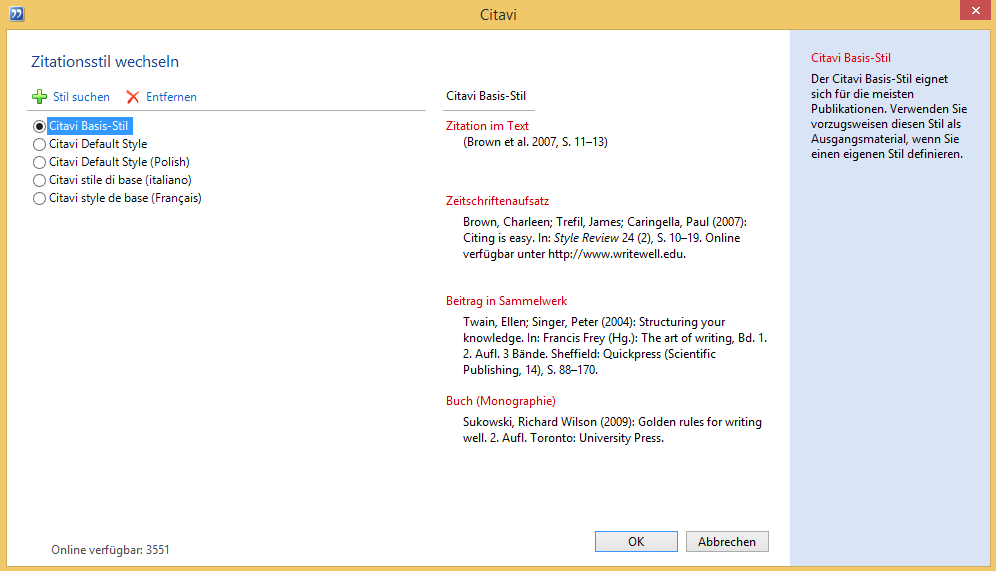
\includegraphics[scale=0.45]{Bilder/Citavi.png}
\end{figure}

Zitate sind grundsätzlich in den Fließtext einzufügen. Fußnoten werden für Zitate nicht genutzt. Nur wenn eine Einbindung der Information in den Text nicht möglich oder sinnvoll ist, kann eine Fußnote genutzt werden. Direkte Zitate sollten vermieden, stattdessen indirekte Zitate bevorzugt werden. Inhalte von Fußnoten sollten möglichst in den Text eingearbeitet werden.
$\;$\\
\begin{spacing}{1}
\textbf{Beitrag in einem Sammelband}\\

Beispiel Literaturangabe:\\

Degele, Nina (2005): Neue Kompetenzen im Internet. In: Kai Lehmann und Michael Schetsche (Hg.): Die Google-Gesellschaft. Wissen im 21. Jahrhundert. Bielefeld: transcript, S. 63–74. \\

\textbf{Buch (Monographie)}\\

Beispiel Literaturangabe:\\

Andretta, Susie; Dervall, John; Li, Han (2005): Information literacy. A practitioner's guide. Oxford: Chandos (Chandos information professionals series). \\

\textbf{Hochschulschrift}\\

Beispiel Literaturangabe:\\

Zweifel, Aron (2005): Information Literacy Konzeption eines Teaching Library-Moduls am Beispiel der Fachhochschulbibliothek Frankfurt am Main. Diplomarbeit. Fachhochschule Frankfurt a. M., Frankfurt a.M. Online verfügbar unter\\ www.fh-frankfurt.de/de/.media/bibliothek/aronzweifel-ilkonzeption-tlmoduls-fh-ffm.pdf, zuletzt geprüft am 30.01.2009.\\

\textbf{Internetdokument}\\

Beispiel Literaturangabe:\\

Arbeitsgemeinschaft Informationskompetenz NRW (2005): ULB Bonn - AG Informationskompetenz - Schulungs- und Lernmaterialien. Online verfügbar unter\\ www.informationskompetenz.de, zuletzt aktualisiert am 24.04.2005, zuletzt geprüft am\\ 30.01.2009.\\
\end{spacing}

Internetzitate werden analog zu den direkten und indirekten Zitaten genutzt. Eine Internetquelle ist nur dann zu zitieren, wenn ein Autor und ein Erscheinungsjahr für die Quelle verfügbar sind.\\

\begin{spacing}{1}

\textbf{Zeitschriftenaufsatz}\\

Beispiel Literaturangabe:\\

Correia, Ana Maria Ramalho; Teixeira, José Carlos (2003): Information literacy. An integrated concept for a safer Internet. In: Online Information Review 27 (5), S. 311–320.\\

\textbf{Zitation im Text:}\\

Beispiele:\\

Ein Autor: (Degele 2005, S. 63)\\
Zwei Autoren: (Correia und Teixeira 2003, S. 319)\\
Ab drei Autoren: (Andretta et al. 2005, S. 5)\\

\end{spacing}

Jedes Werk, aus dem zitiert wurde, muss im Literaturverzeichnis aufgeführt werden. Werke, die zur Erarbeitung des Themas genutzt aber nicht zitiert wurden, gehören nicht ins Literaturverzeichnis. \\

Die Universitätsbibliothek bietet Ihnen mit dem Literaturverwaltungsprogramm RefWorks ebenso ein persönliches und kostenfreies Tool für die professionelle Verwaltung Ihrer Literaturangaben. Weitere Informationen finden sich auf der Uni-Homepage:\\http://www.bibliothek.uni-augsburg.de/service/literaturverwaltung/refworks/









\clearpage


\subsection{Der Schreib- und Forschungsprozess}

\begin{figure}[h]
\centering
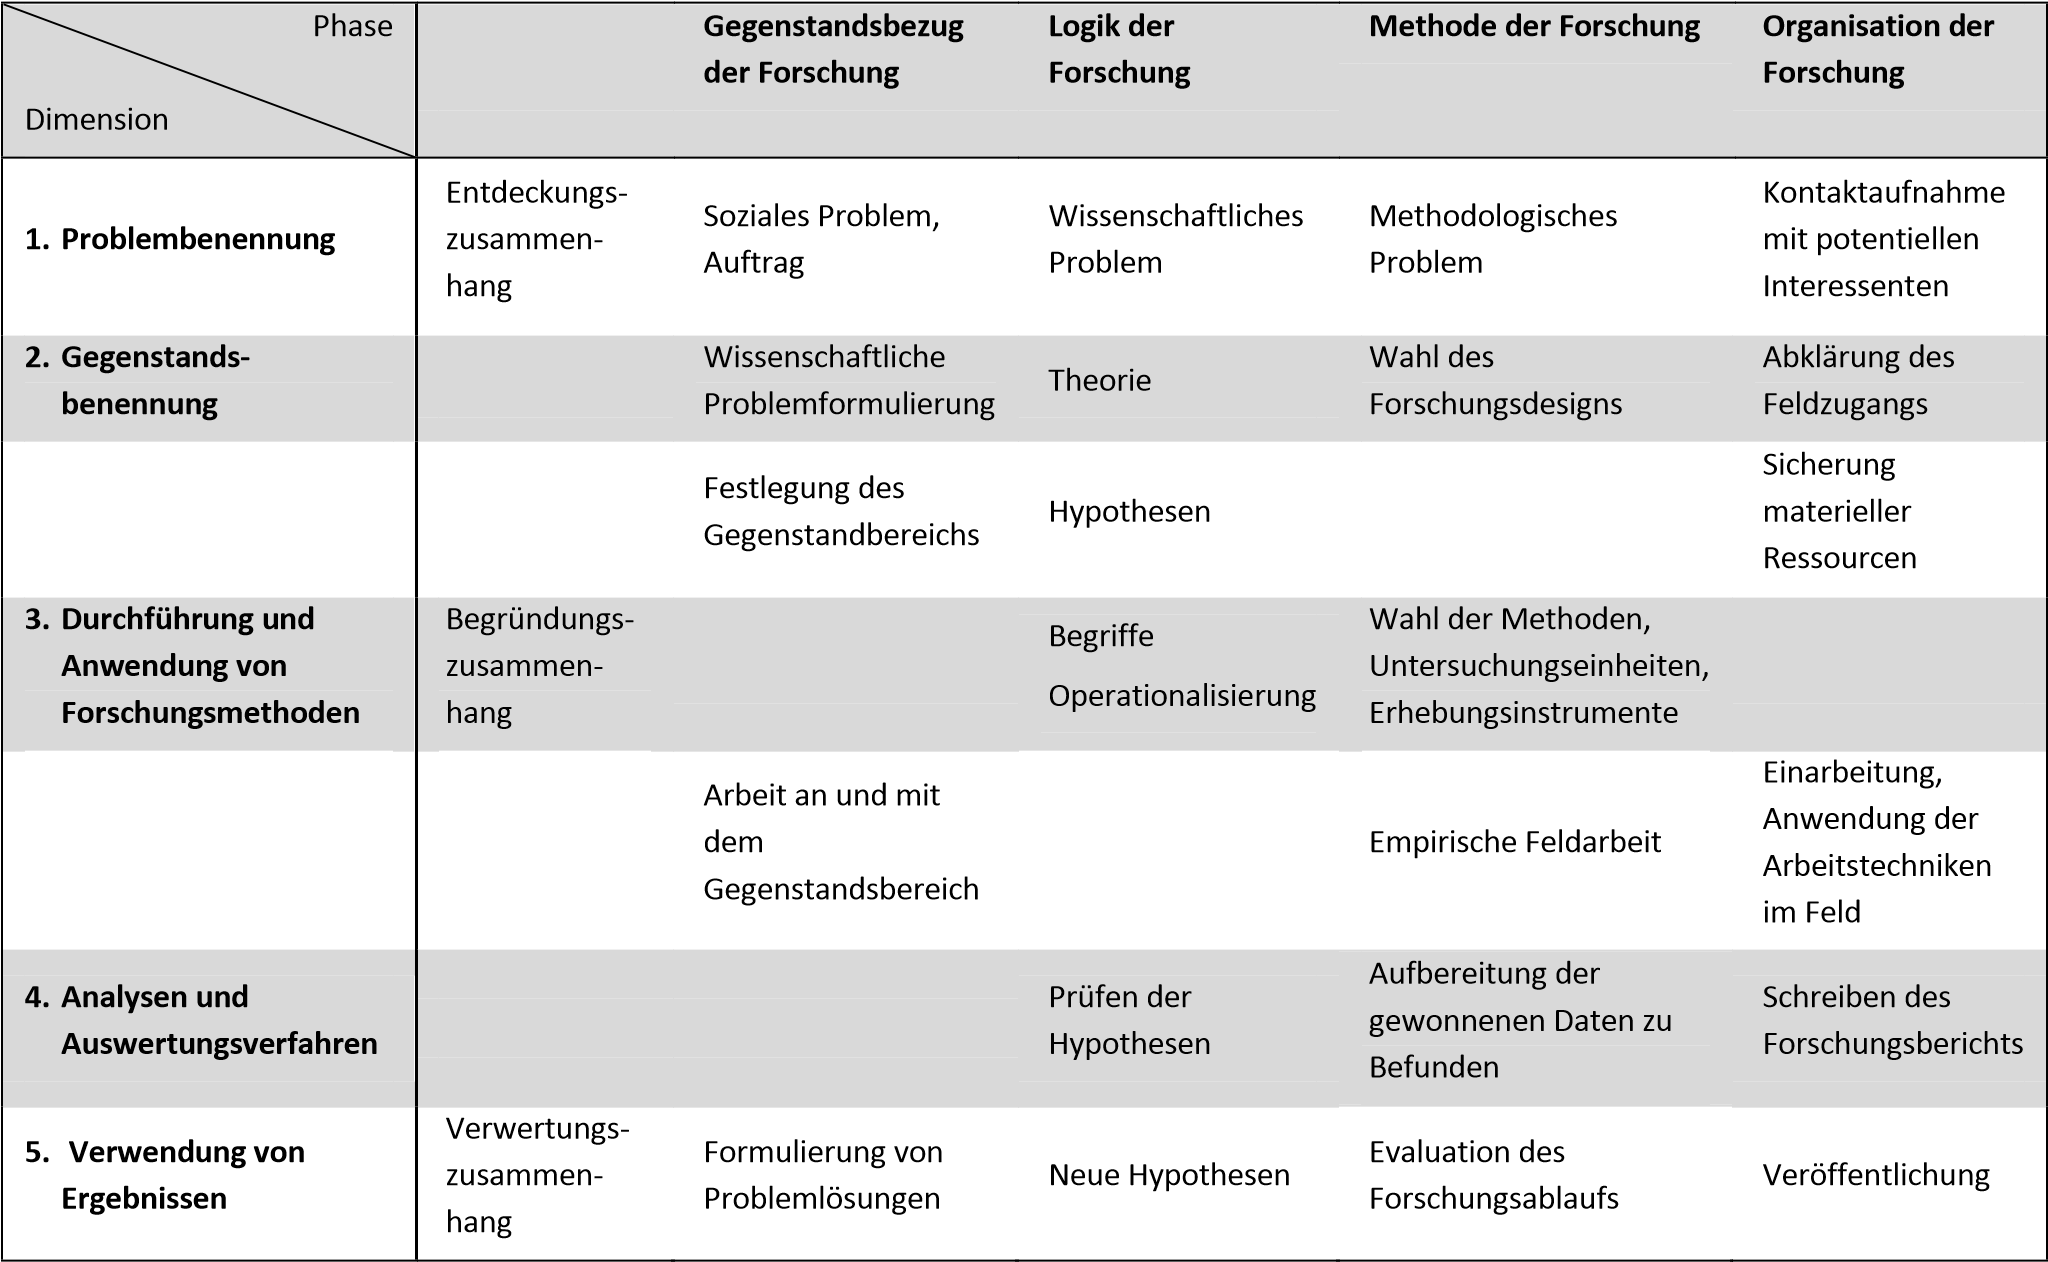
\includegraphics[width=1\textwidth]{Bilder/Abbildung.png}
Quelle: \citet{atteslander2010}, S. 13
\caption{Dimension einer wissenschaftlichen Arbeit nach Peter Atteslander}
\label{abb:abbildung1}
\end{figure}










\clearpage



\subsection{Bestandteile einer wissenschaftlichen Arbeit}


\begin{table}[htbp]
\renewcommand{\arraystretch}{1.4} 
  \centering

    \begin{tabular}{|l|l|}
\hline
    \textbf{{\large Hauptgruppe}} &  \textbf{{\large Bestandteile}} \\  \hline
    Titel &  $\cdot \quad$ Titelblatt \\ \hline
    Einleitungsapparat &  $\cdot \quad$ Abstract \\
	& $\cdot \quad$ Inhaltsverzeichnis \\
          &  $\cdot \quad$ Abbildungsverzeichnis \\
          &  $\cdot \quad$ Tabellenverzeichnis \\
	&  $\cdot \quad$ Abkürzungsverzeichnis \\ \hline
    Einführung &  $\cdot \quad$ Kurze Hinführung zum Thema \\ \hline
    Hauptteil &  $\cdot \quad$ Detaillierte Behandlung des Themas  \\ \hline
    Schluss &  $\cdot \quad$ Zusammenfassung und Ausblick \\ \hline
    Abschlussapparat & $\cdot \quad$ Anhang \\
	& $\cdot \quad$ Literaturverzeichnis \\
          &  $\cdot \quad$ Eidesstattliche Erklärung \\ \hline

    \end{tabular}%
  \label{tab:tabelle1}%



$\;$\\

\caption{Bestandteile einer wissenschaftlichen Hausarbeit}

Quelle: \citet{atteslander2010}, S. 13

\end{table}
Tabellen und Abbildungen unterstreichen Aussagen und illustrieren Forschungsergebnisse, um deren Verständnis für den Leser zu erleichtern. Sie dürfen nur dann eingesetzt werden, wenn sie im Text ausführlich erläutert werden. Bitte achten Sie darauf, dass die Tabellen selbsterklärend und notwendige Inhalte in die Tabellenbeschreibung aufzunehmen sind. Qualitativ müssen alle Abbildungen und Tabellen so hochwertig sein, dass sie sowohl auf dem Bildschirm, als auch auf einem Ausdruck klar und deutlich lesbar sind. Formal benötigt jede Abbildung eine Abbildungsunterschrift, jede Tabelle eine Tabellenüberschrift. Außerdem ist jeweils eine Quellenangabe, entsprechend der Zitation im Text, anzufügen.\\
Stilistisch ist auf eine neutrale Formulierung zu achten. Formulierungen mit „ich, man, wir, es“ sollten unbedingt vermieden werden.












\clearpage
\section{Riemanns Beweis}
\label{sec:kapitel3}

Wenden wir die Poisson-Summenformel f\" ur $\kinf$ auf die Schwartz-Funktion $\ginf(\xinf):=e^{-\pi|\xinf|^2}$ an, sehen wir, dass die Thetafunktion
\begin{align}
	\Theta_\infty (\xinf):=\sum_{n\in\Z}{\ginf (n\xinf)} = 1+ 2\sum_{n=1}^\infty{e^{-\pi n^2 |\xinf|_\infty^2}}
\end{align}
die Funktionalgleichung
\begin{align}
	\label{eq:thetafunktional}
	\Theta_\infty (\xinf) = \frac{1}{|\xinf|_\infty} \Theta_\infty(\frac{1}{\xinf})
\end{align}

f\"ur $\xinf \in \kinf^\times :=\kinf\setminus{0}$. Da insbesondere $\Theta_\infty(x_\infty)-1$ f\"ur $\xinf \rightarrow \infty$ schnell f\"allt, sehen wir, dass $\Theta_\infty(\xinf) - 1 / \xinf$ schnell f\"allt wenn $\xinf \rightarrow 0$. 
Formal k\"onnen wir die Mellin-Transformation auf \eqref{eq:thetafunktional} anwenden und folgern
\begin{align}
	\label{eq:thetamellin}
	\int_{k_\infty^\times} \Theta_\infty(x_\infty) |x_\infty|_\infty^s d^\times x_\infty = \int_{k_\infty^\times} \Theta_\infty(x_\infty) |x_\infty|_\infty^{1-s} d^\times x_\infty
\end{align}

f\"ur beliebige $s$, wobei $d^\times x_\infty := \frac{dx_\infty}{|x_\infty|_\infty}$ das standard multiplikative Haarma{\ss} auf $\kinf^\times$ ist. Dies macht streng genommen keinen Sinn, da die beiden Integranden hier bei $0$ und $\infty$ divergieren (was letztendlich auf die Pole der Riemannschen Xi Funktion bei $s=0$ und $s=1$ zur\"uckgeht). Setzen wir hier trotzdem weiter an. Verwenden wir den Trafo $y := \pi n^2 t^2$ und erinnern uns an die Formeln der Riemannschen Xi Funktion und des Gamma-Faktors, erhalten wir
\begin{align}
	 \int_{k_\infty}e^{-\pi n^2 x_\infty^2} |x_\infty|_\infty^s d^\times x_\infty = \Gamma_\infty(s) n^{-s}
\end{align}

und somit formal
\begin{align}
	\int_{k_\infty} \Theta_\infty(x_\infty) |x_\infty|_\infty^s d^\times x_\infty = \int_{k_\infty} |x_\infty|^s d^\times x_\infty + 2\Gamma_\infty(s) \zeta(s)
\end{align}

Schmei{\ss}en wir das divergente Integral $\int_{k_\infty} |x_\infty|^s d^\times x_\infty$ weg und wenden \eqref{eq:thetamellin} erhalten wir rein formal die Funktionalgleichung \eqref{eq:funktionalgleichung}. Diese Berechnungen waren nur formeller Natur.

Dieser Teil soll die Arbeit abrunden und ein kurzes Fazit liefern.
\clearpage




\bibliographystyle{plain_literaturverzeichnis}
\bibliography{literatur}
\clearpage




\appendix

\section{Anhang}
\label{sec:anhang}

\large\textbf{Anhang 1: Beschreibung}\\
\normalsize
Sie können an dieser Stelle (fortlaufend nummeriert und jeweils mit Seitenumbruch getrennt) Inhalte einfügen, die zum Verständnis der Arbeit nicht kritisch sind, jedoch Teil des Gesamtwerks sein sollen.






\clearpage





\thispagestyle{empty}
\section*{Eidesstattliche Erklärung}
Ich/Wir versichere/versichern, dass ich/wir die vorliegende Arbeit ohne fremde Hilfe und ohne Benutzung anderer als der angegebenen Quellen angefertigt habe, und dass die Arbeit in gleicher oder ähnlicher Form noch keiner anderen Prüfungsbehörde vorgelegen hat. Alle Ausführungen der Arbeit, die wörtlich oder sinngemäß übernommen wurden, sind als solche gekennzeichnet.\\
\linebreak
\linebreak
\flushleft
[Name, Vorname, Unterschrift (entfällt bei online-Dokumenten)]
\flushleft
[Ort, Datum]
\clearpage

\end{spacing}





























\end{document}

